\chapter{CONCLUSION AND FURTHER DEVELOPMENT}
\label{chap:relatedwork}

In Chapter 6, we describe a few recent works relating to river runoff prediction and boiler efficiency optimization.

\minitoc

\section{Accomplishment}
\section{Limitation}
\section{Further development}
\section{Instruction}
\subsection{Verifying account}
1. Login with your account or register new account. 
\begin{center}
    \begin{figure}[H]
    \centering
    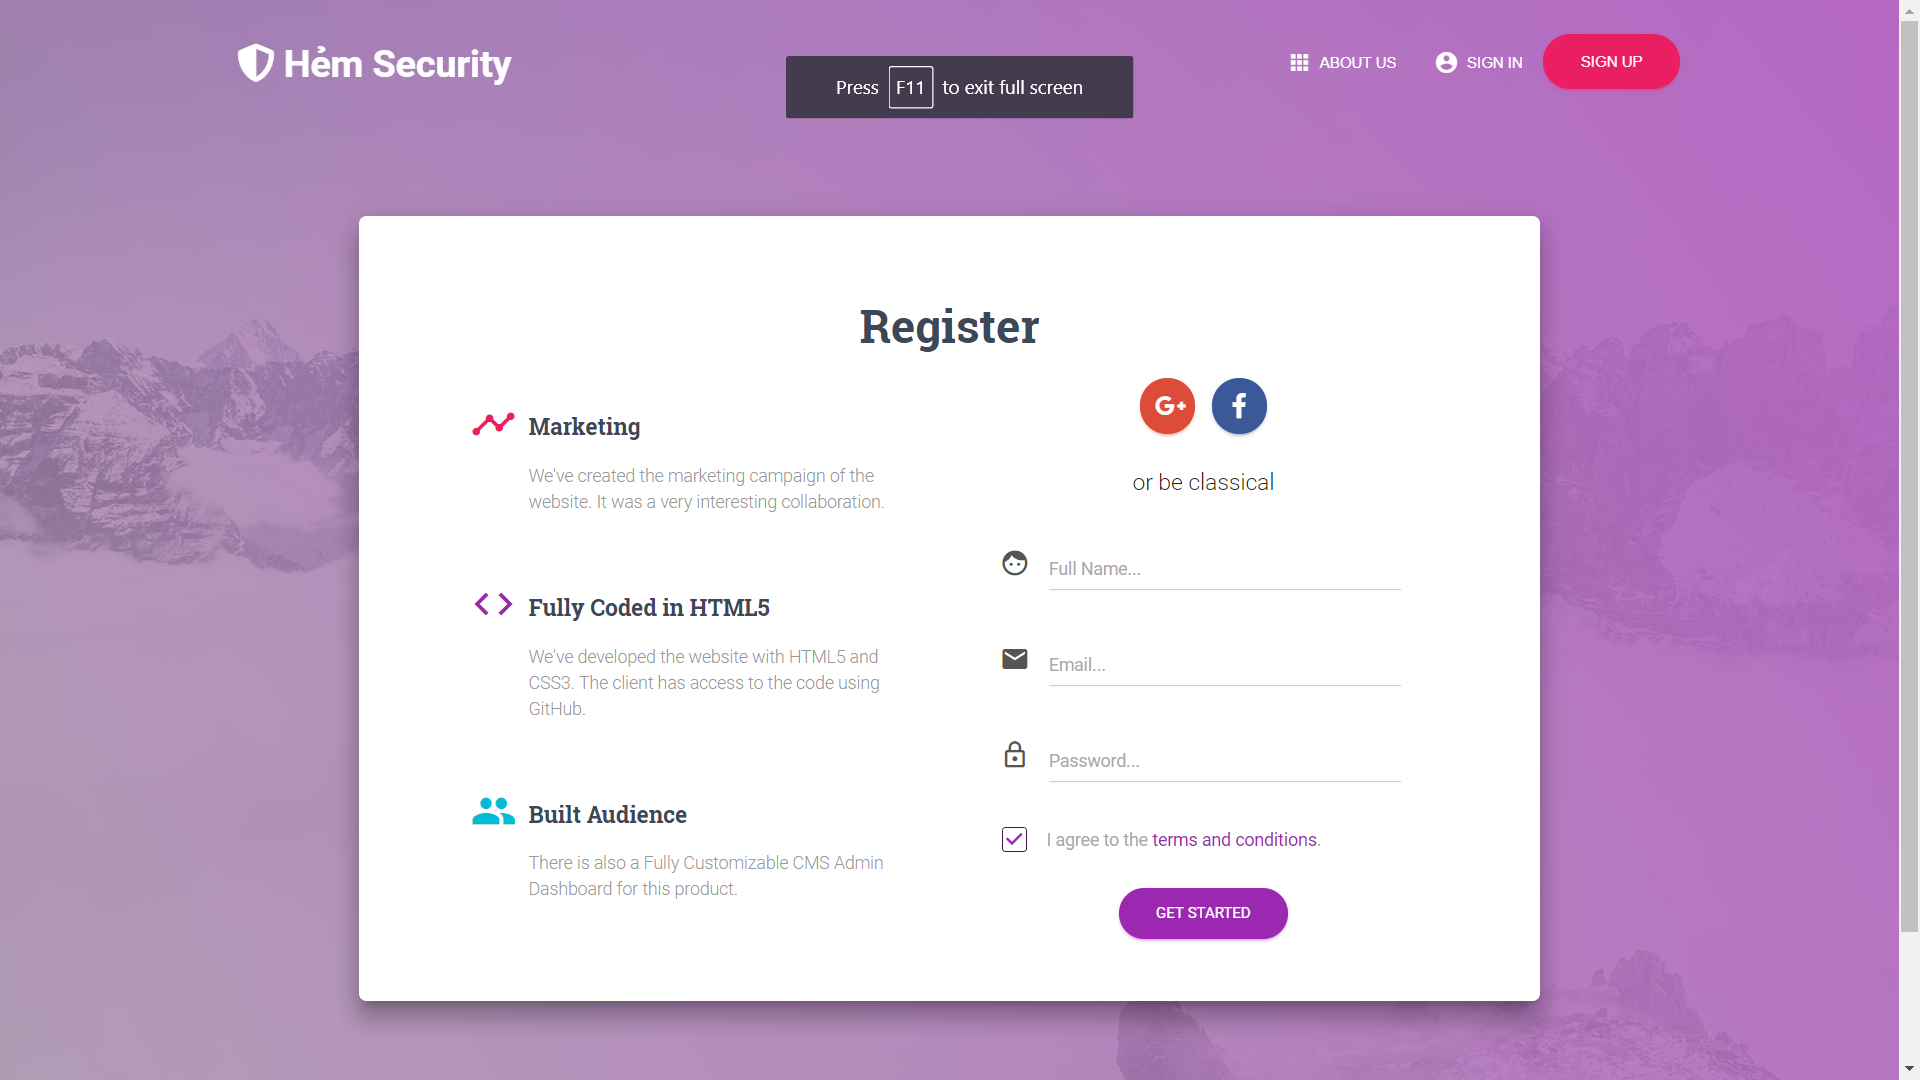
\includegraphics[width=1\columnwidth]{images/chap6/instruction1.png}
    \footcaption{Homepage}
    \label{}
    \end{figure}
\end{center}
2. Unverified account is unable to use most of the features, verify your account by clicking your name to go to your profile page
\begin{center}
    \begin{figure}[H]
    \centering
    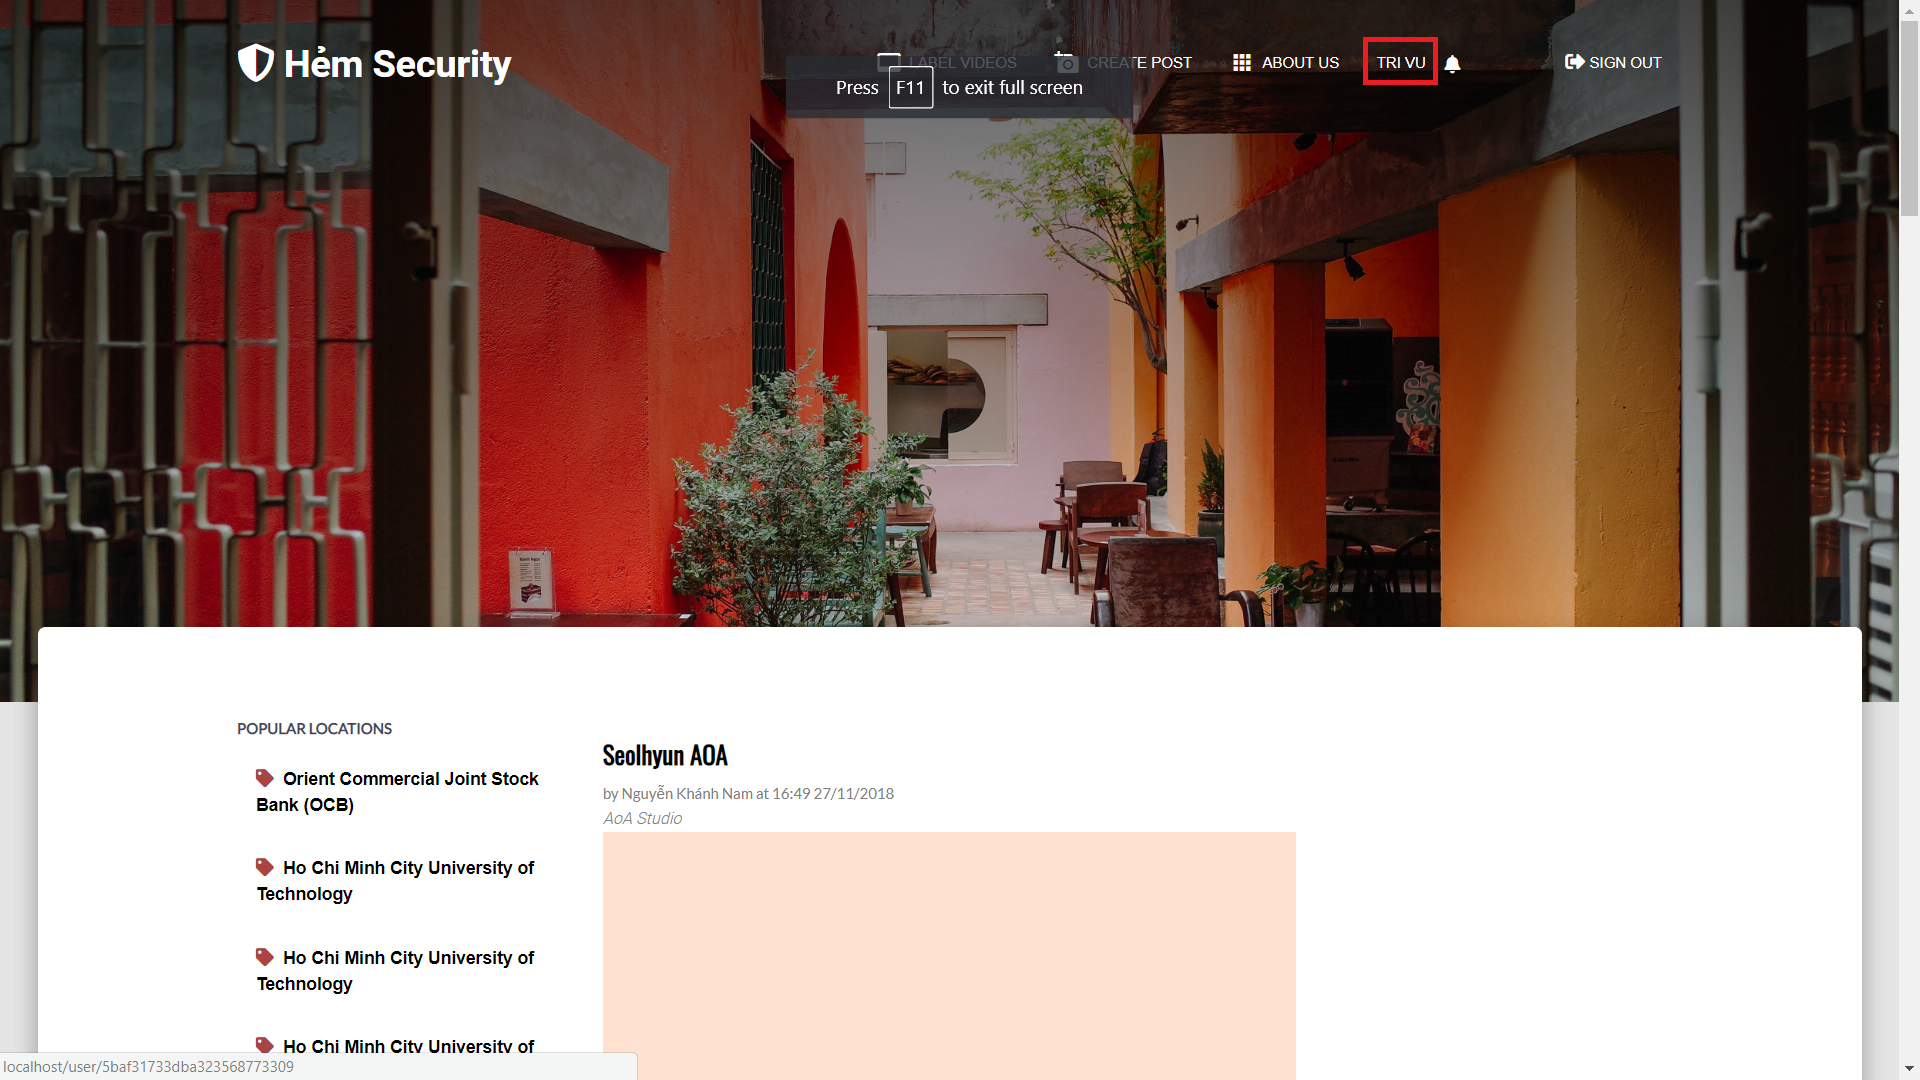
\includegraphics[width=1\columnwidth]{images/chap6/instruction2.png}
    \end{figure}
\end{center}
3. Enter your phone number to verify
\begin{center}
    \begin{figure}[H]
    \centering
    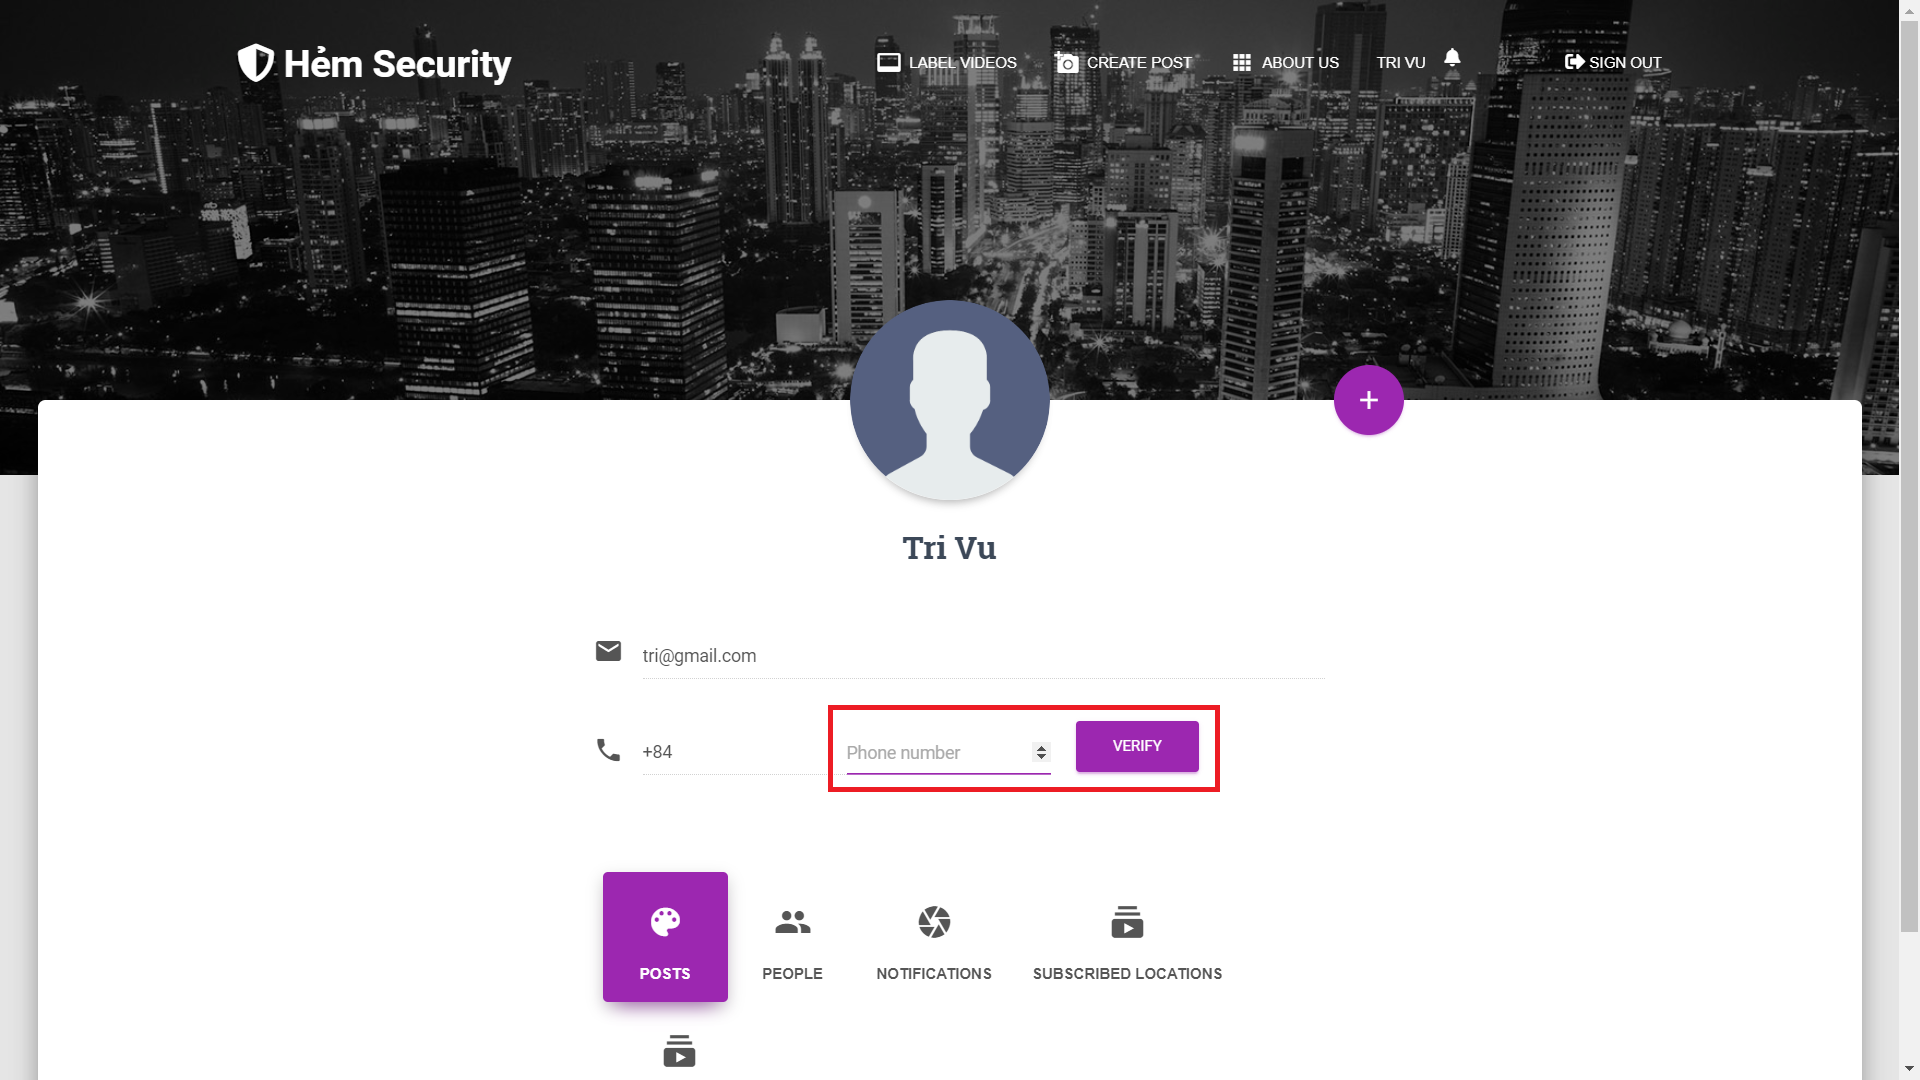
\includegraphics[width=1\columnwidth]{images/chap6/instruction3.png}
    \end{figure}
\end{center}
4. User can choose either to receive confirmation code by WhatsApp or SMS. Enter your code to finish verifying.
\begin{center}
    \begin{figure}[H]
    \centering
    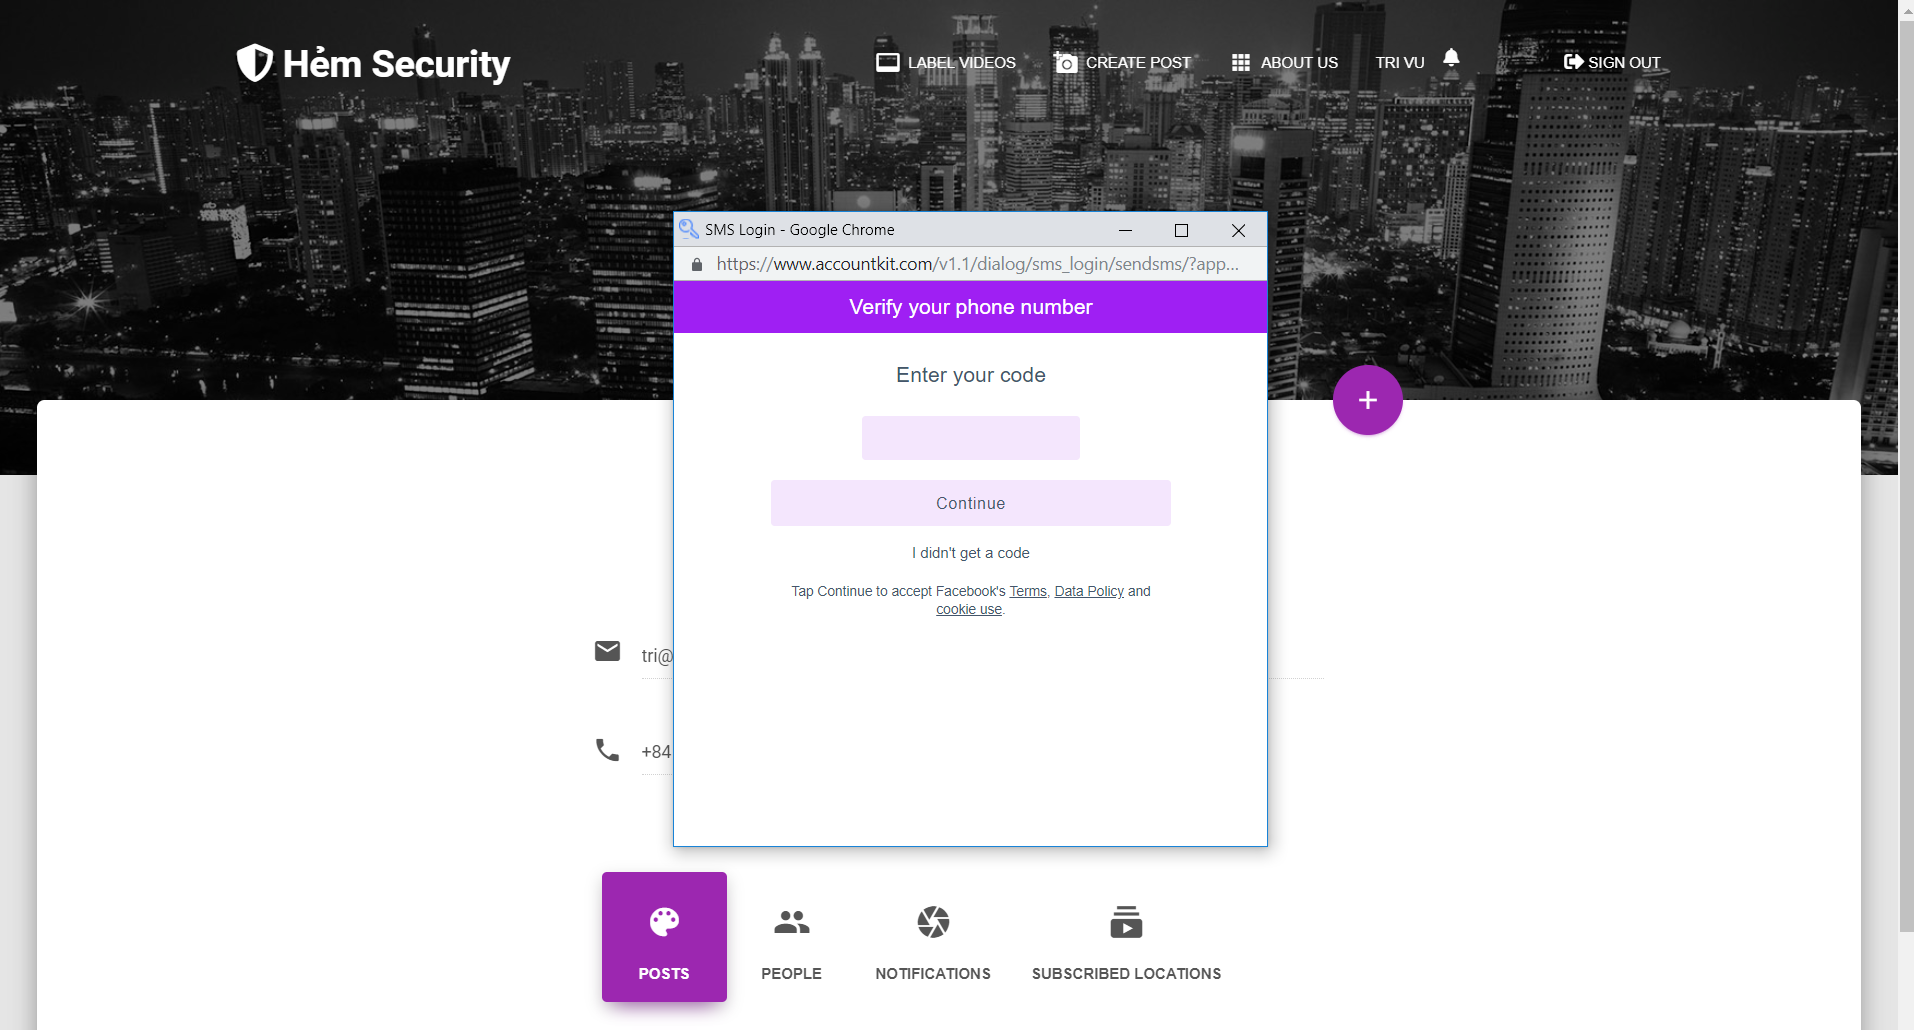
\includegraphics[width=1\columnwidth]{images/chap6/instruction4.png}
    \end{figure}
\end{center}
\subsection{Label video}
1. Go to "Label video" page
\begin{center}
    \begin{figure}[H]
    \centering
    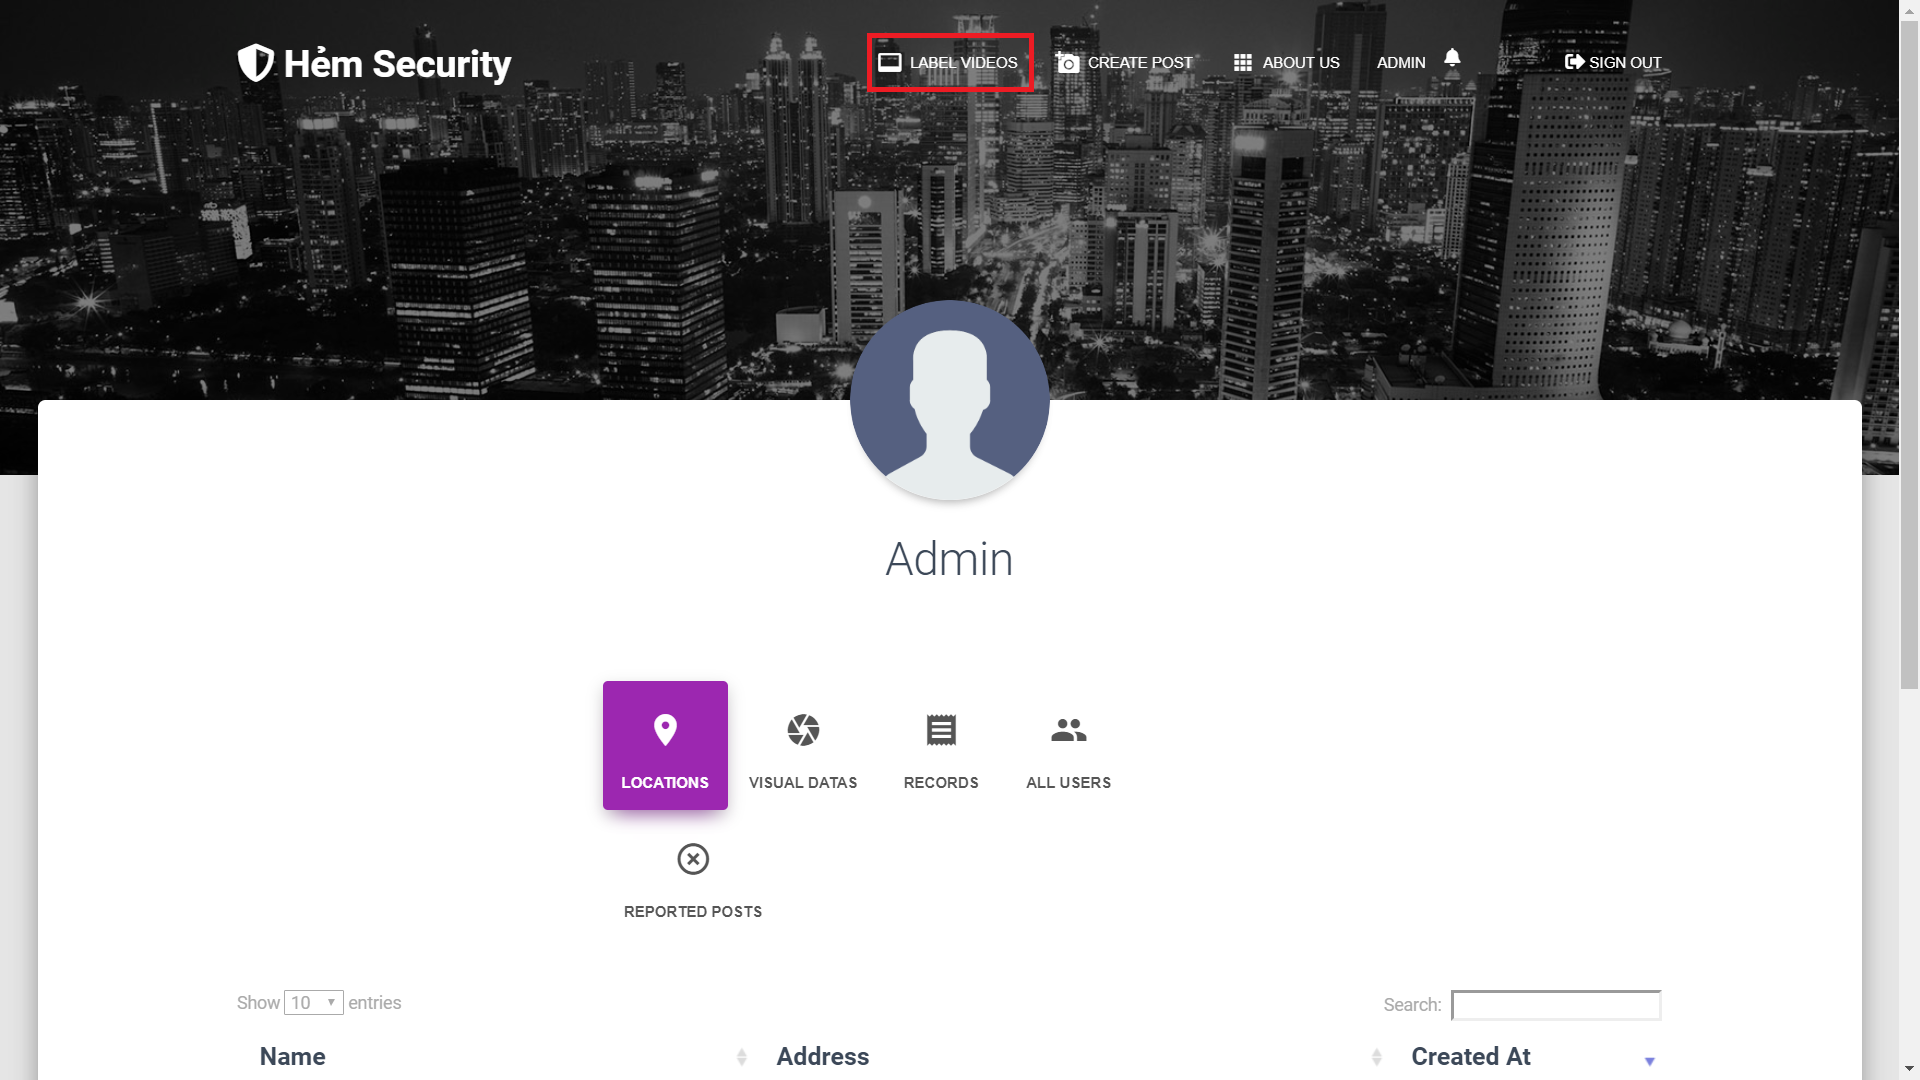
\includegraphics[width=1\columnwidth]{images/chap6/instruction5.png}
    \end{figure}
\end{center}
2. Choose either "Suspicious" or "Not suspicious". 
\begin{center}
    \begin{figure}[H]
    \centering
    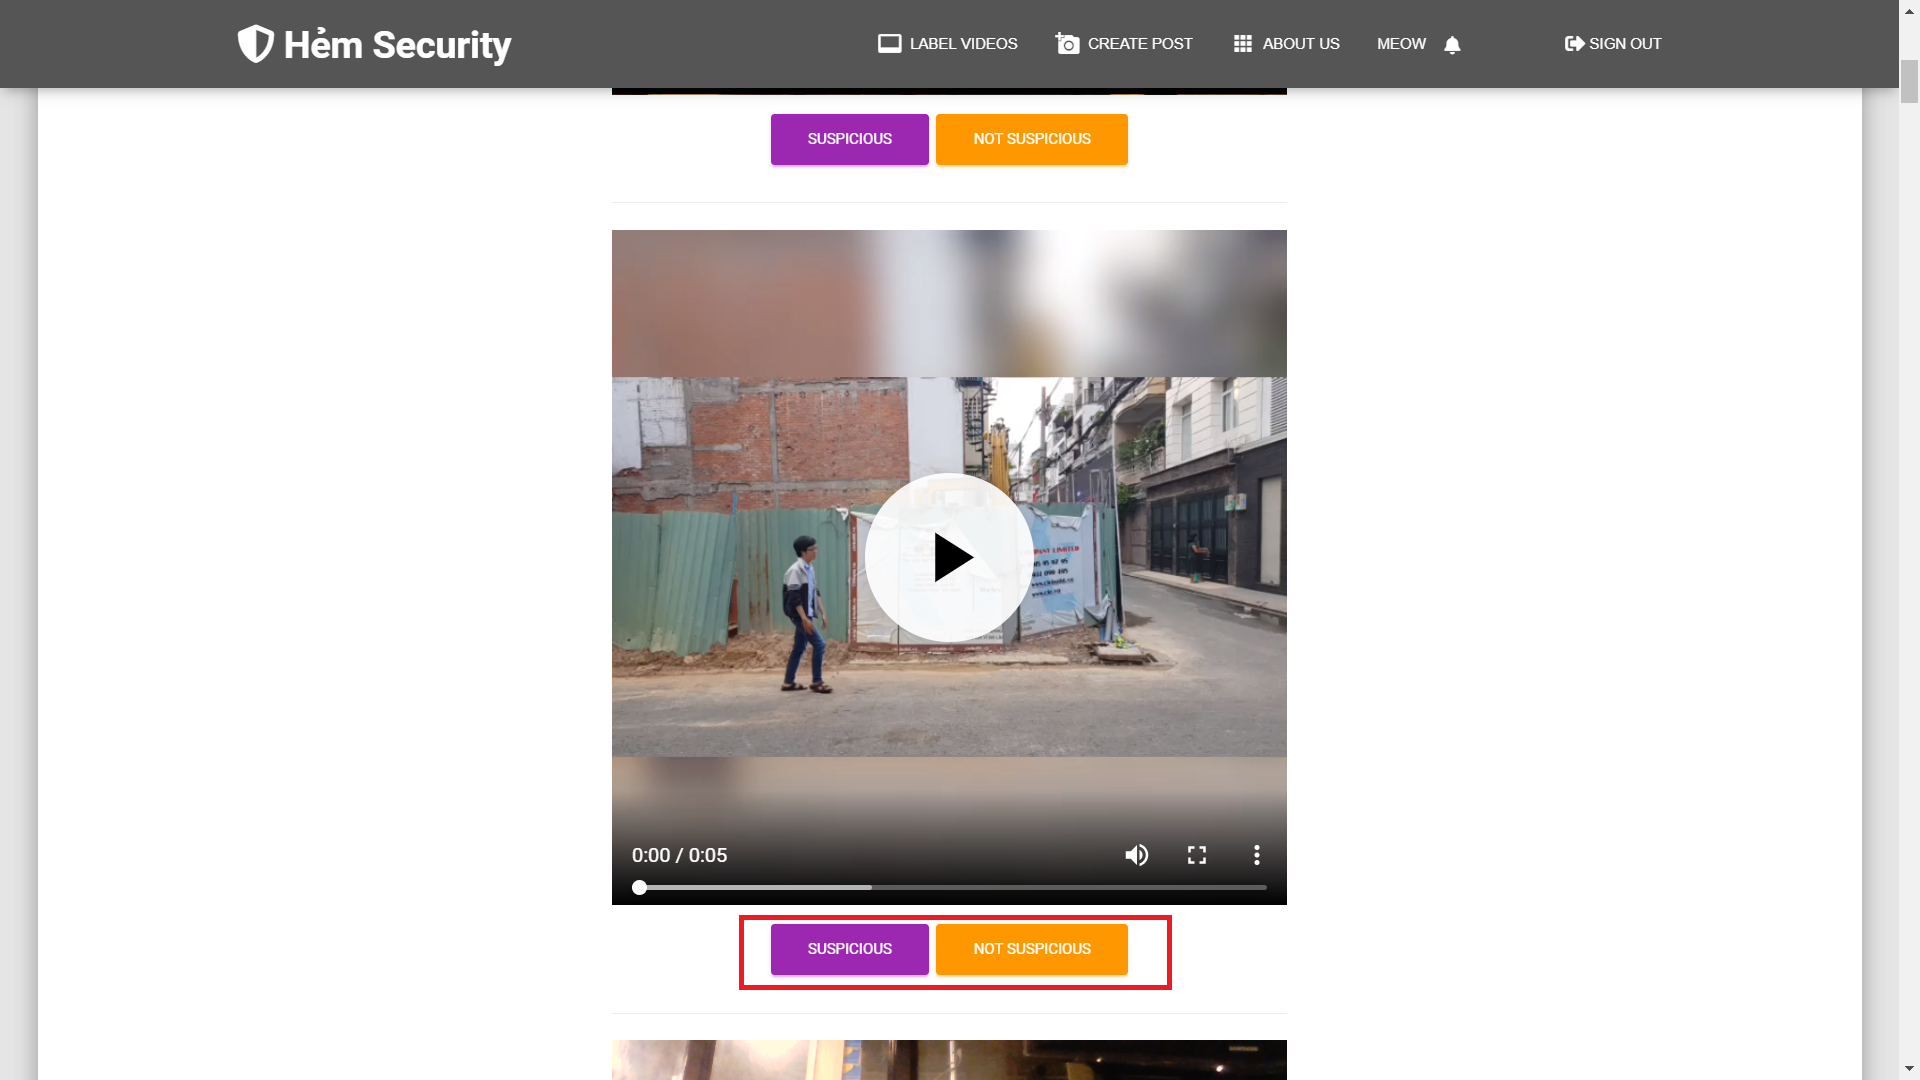
\includegraphics[width=1\columnwidth]{images/chap6/instruction6.png}
    \end{figure}
\end{center}
\subsection{Create post}
1. Go to "Create post" page
\begin{center}
    \begin{figure}[H]
    \centering
    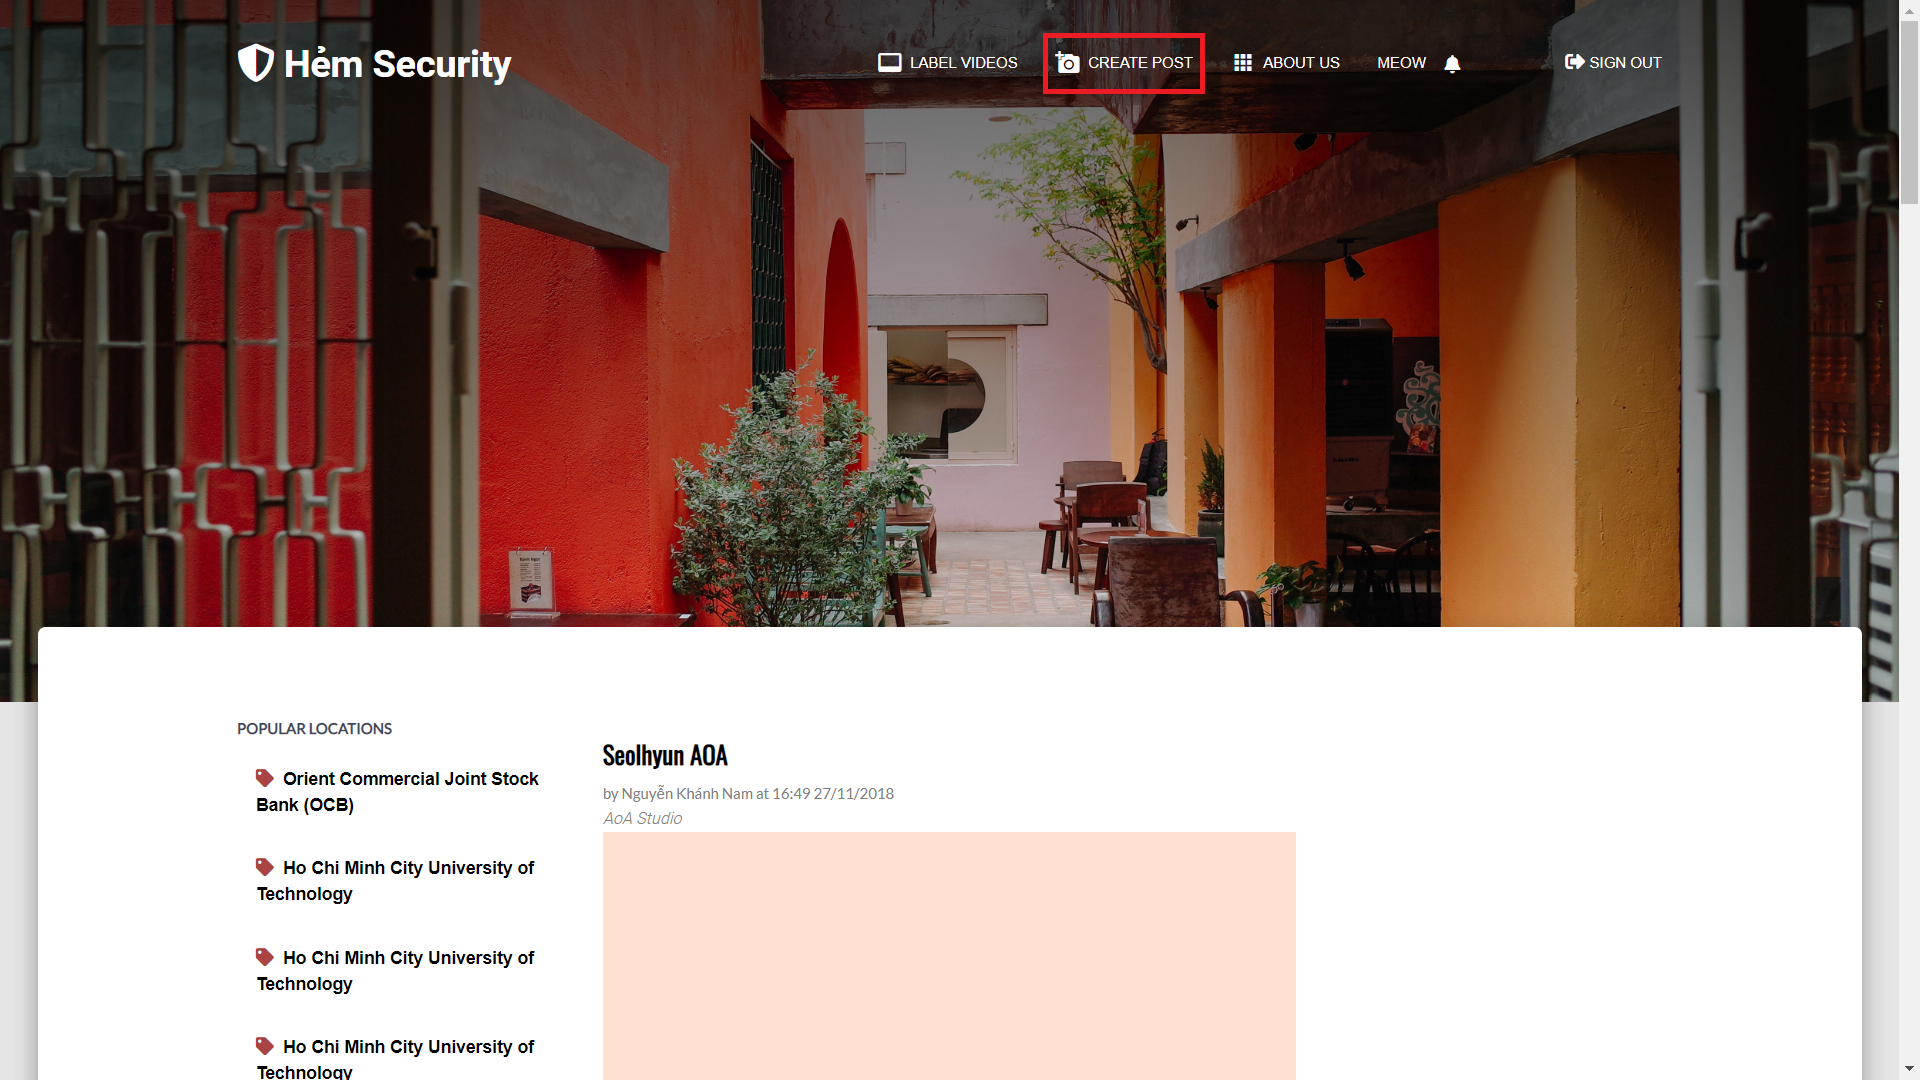
\includegraphics[width=1\columnwidth]{images/chap6/instruction7.png}
    \end{figure}
\end{center}
2. Fill in the form to and click "Create". 
\begin{center}
    \begin{figure}[H]
    \centering
    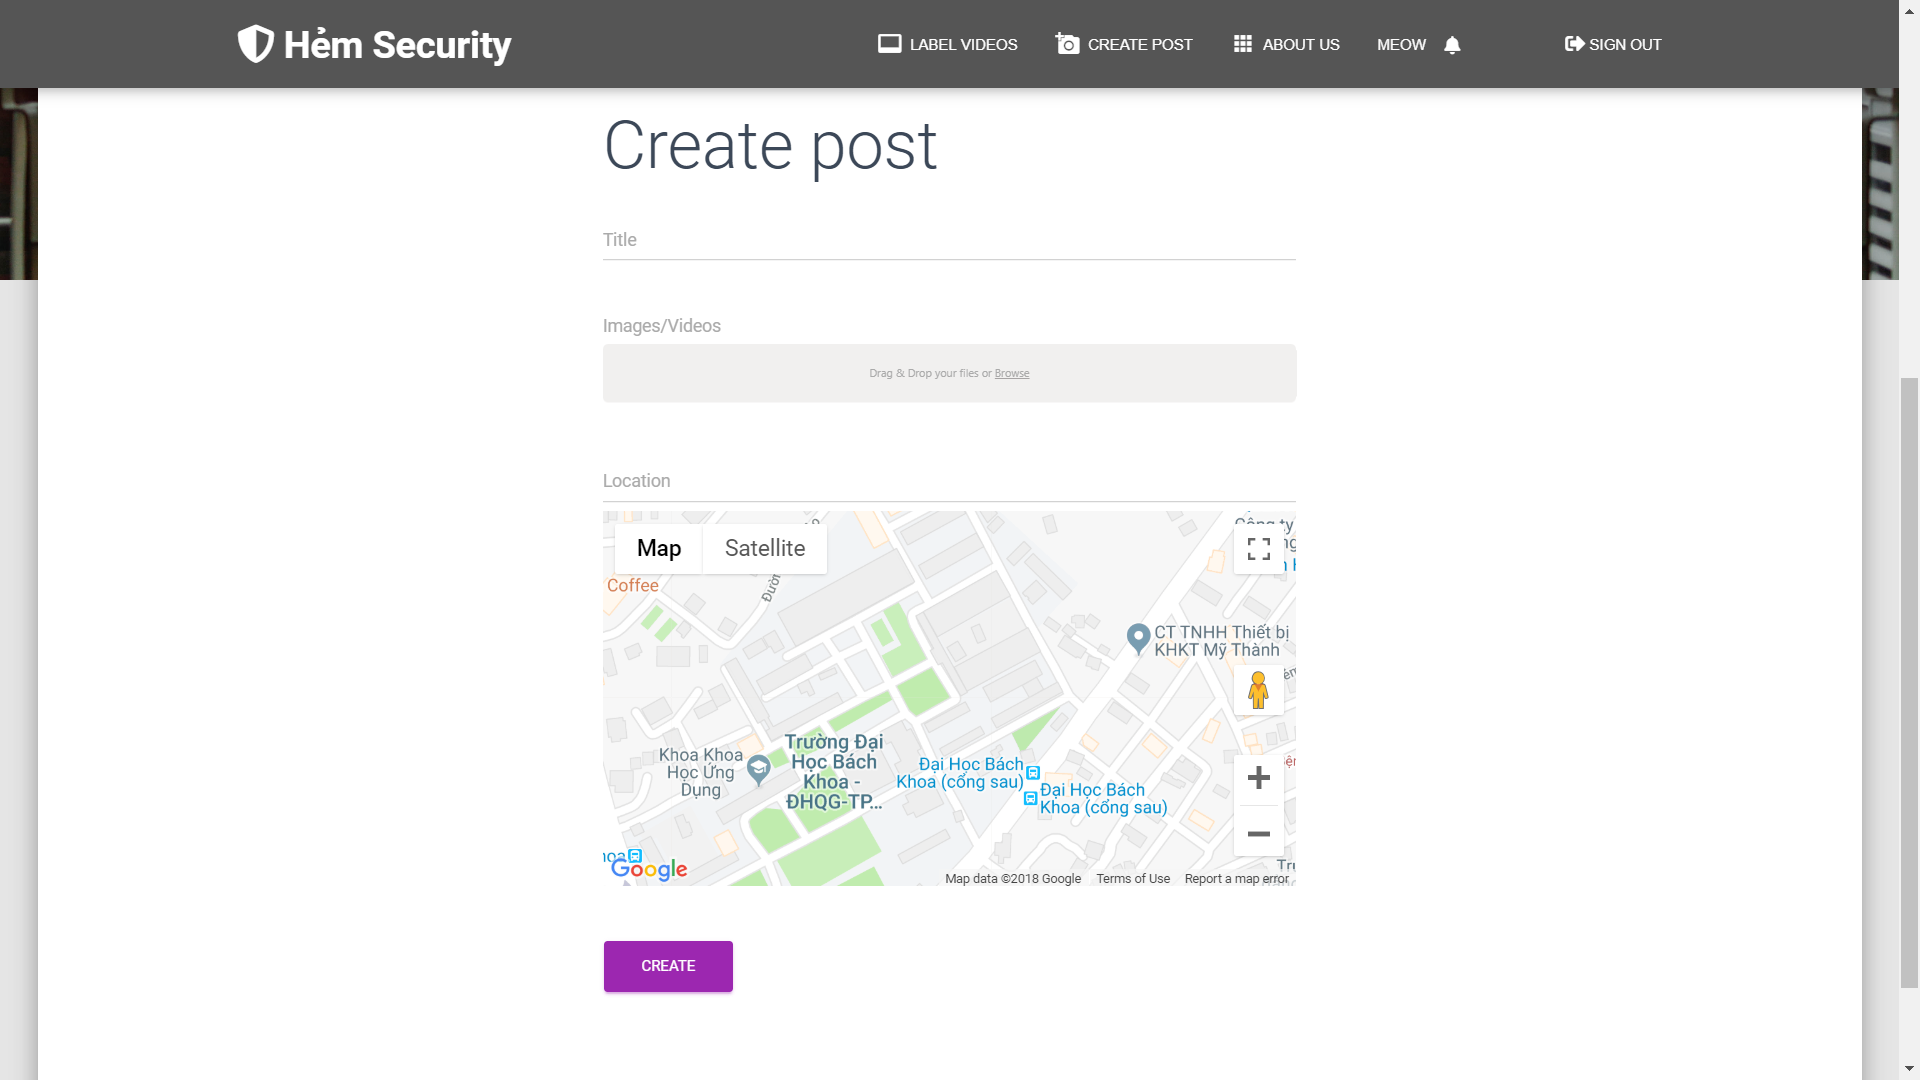
\includegraphics[width=1\columnwidth]{images/chap6/instruction8.png}
    \footcaption{Create post form}
    \end{figure}
\end{center}
\subsection{Subscribe a location}
1. Go to profile page and choose "All locations" tab
\begin{center}
    \begin{figure}[H]
    \centering
    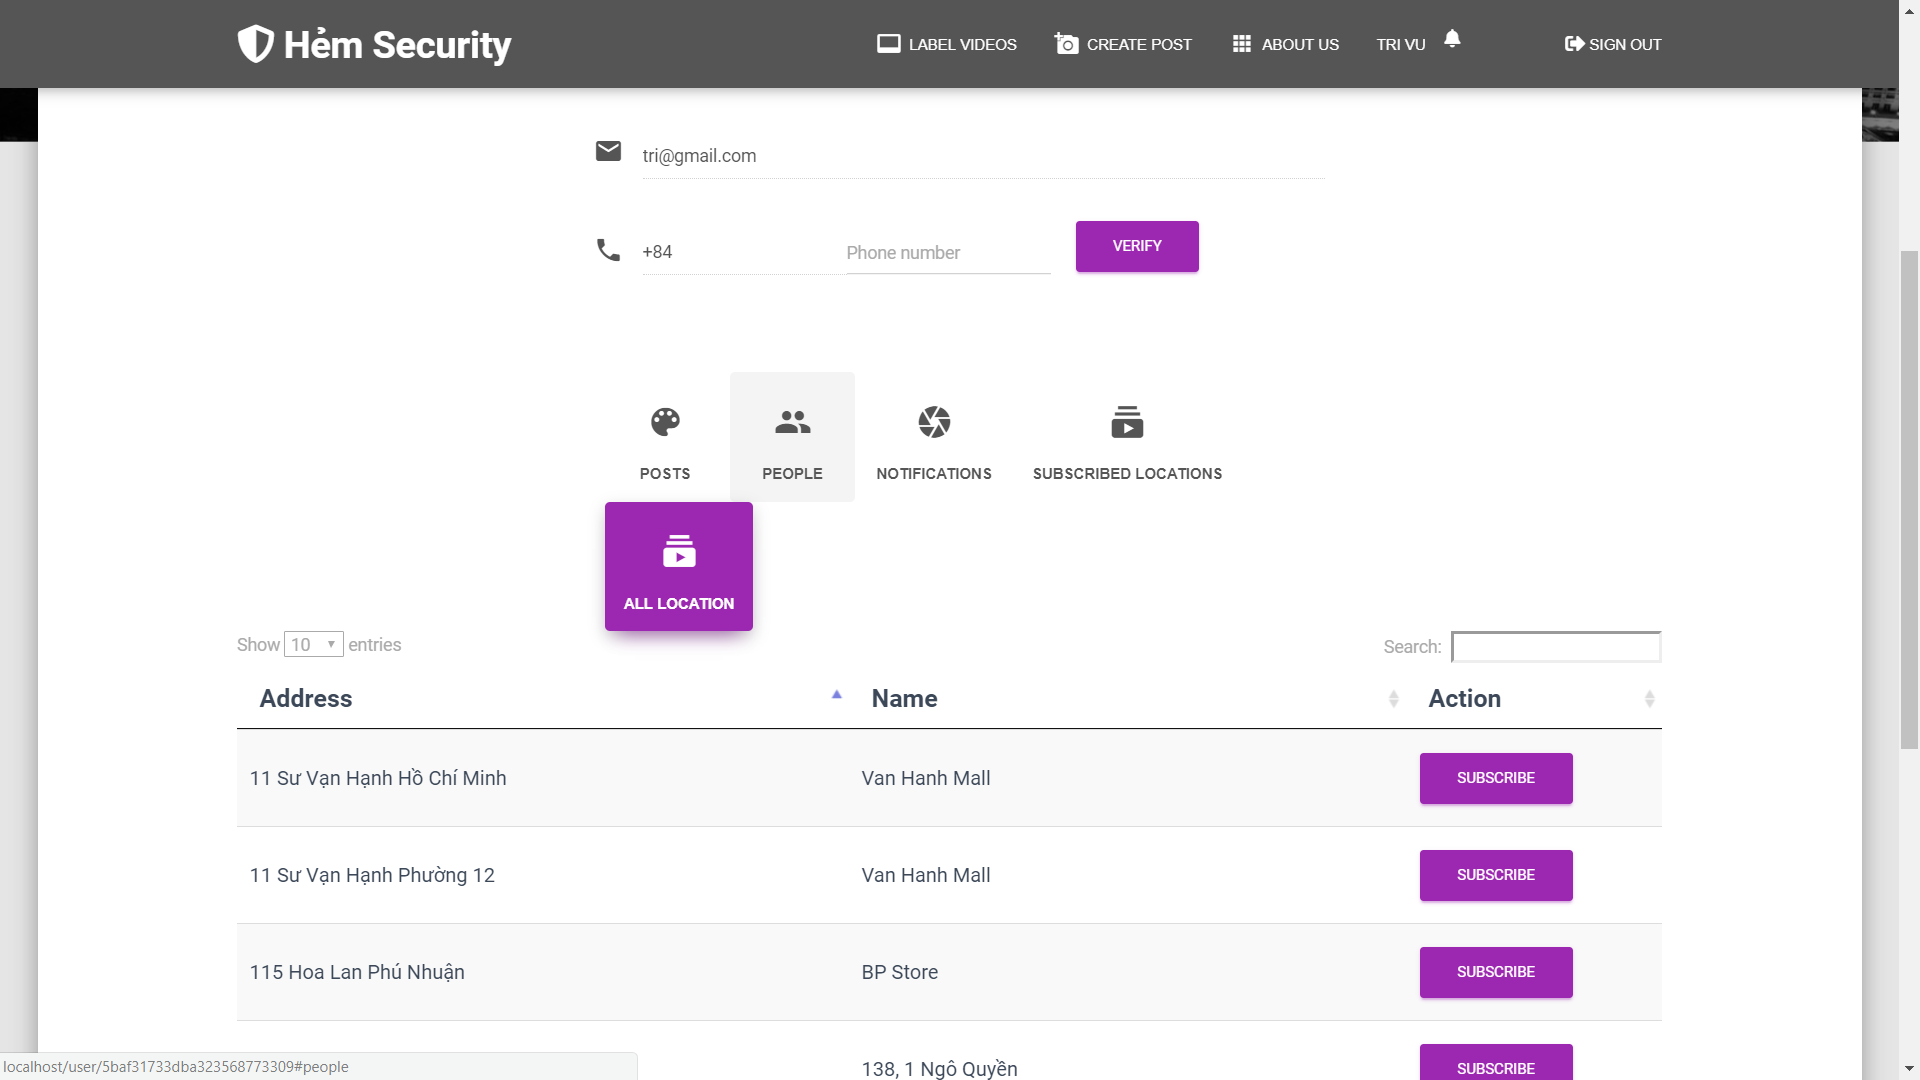
\includegraphics[width=1\columnwidth]{images/chap6/instruction9.png}
    \end{figure}
\end{center}
2. Choose a location to subscribe from the list. User will receive notification about suspicious behavior around subscribed location within a radius of 1 kilometer.   
\begin{center}
    \begin{figure}[H]
    \centering
    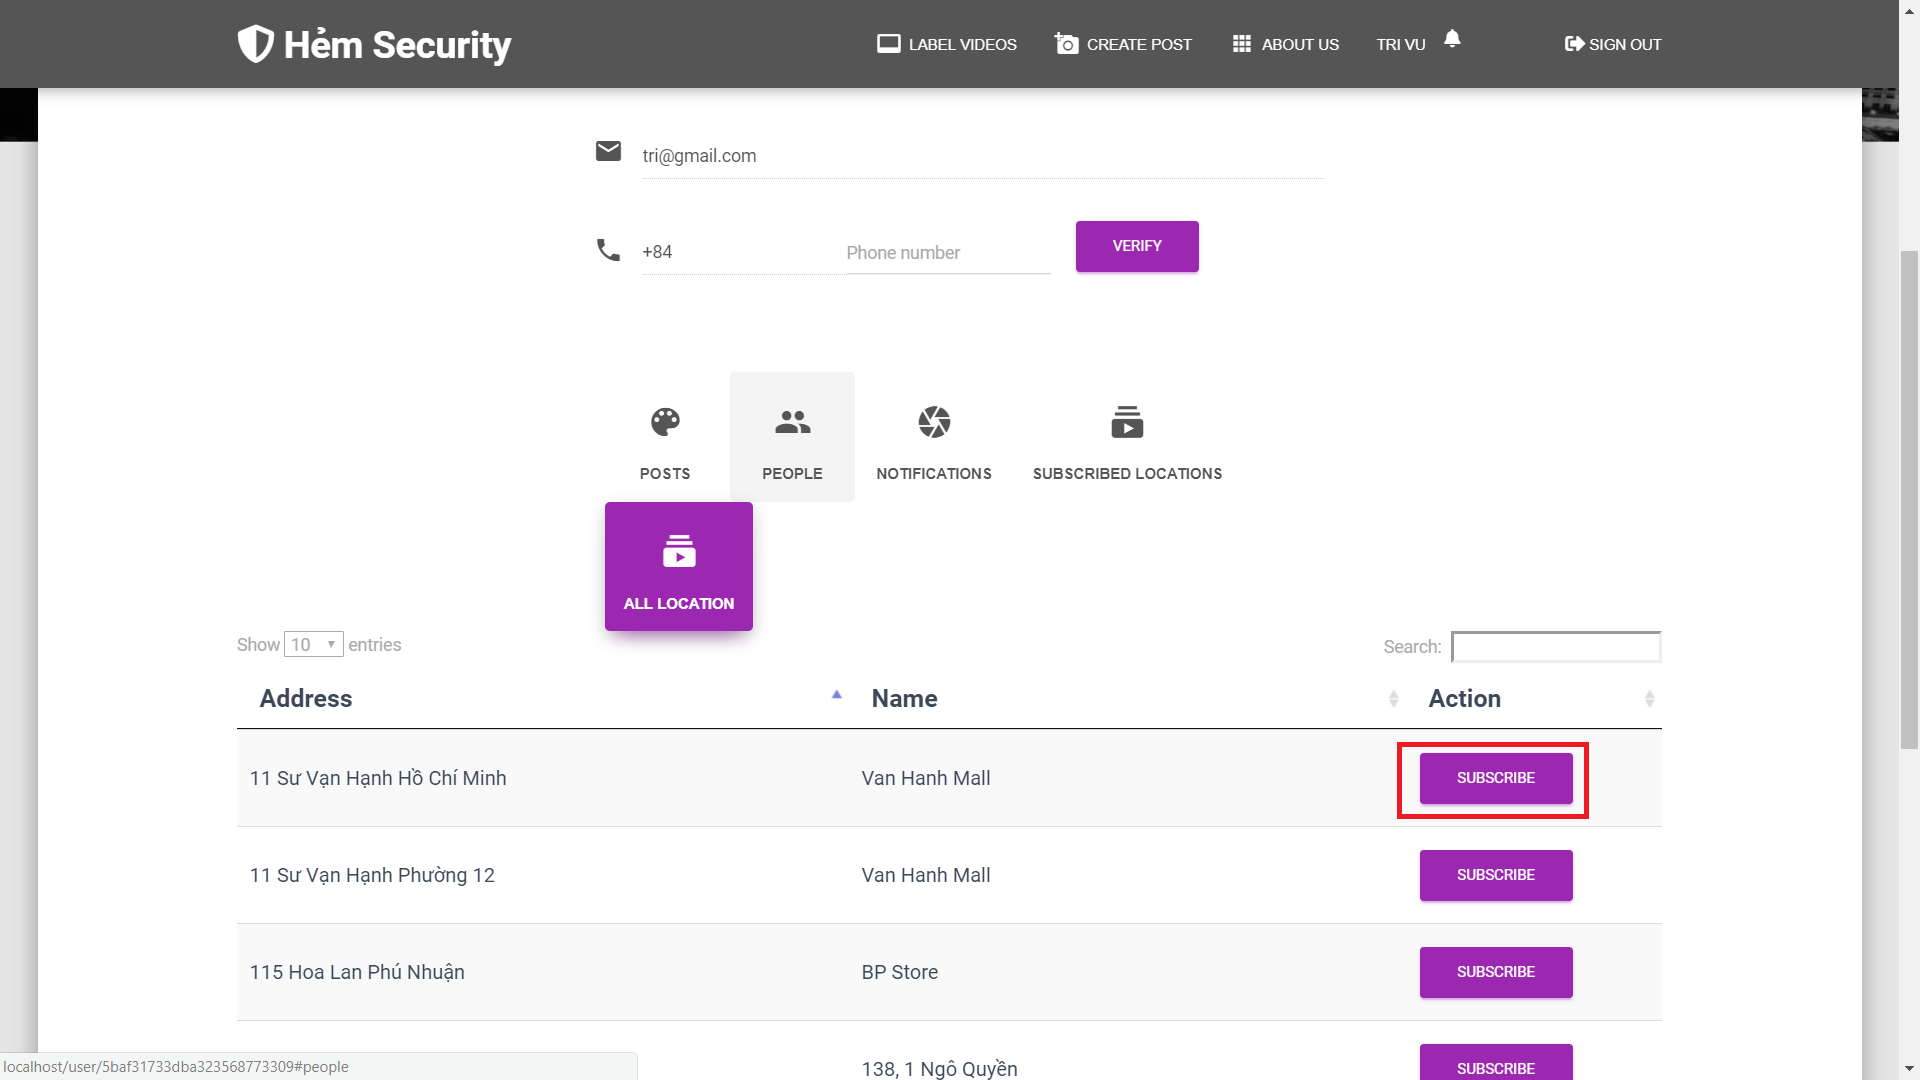
\includegraphics[width=1\columnwidth]{images/chap6/instruction10.png}
    \end{figure}
\end{center}




Hình \ref{chap2:neural_model} mô tả mô hình một neural trong mạng neural nhân tạo.
\begin{center}
    \begin{figure}[H]
    \centering
    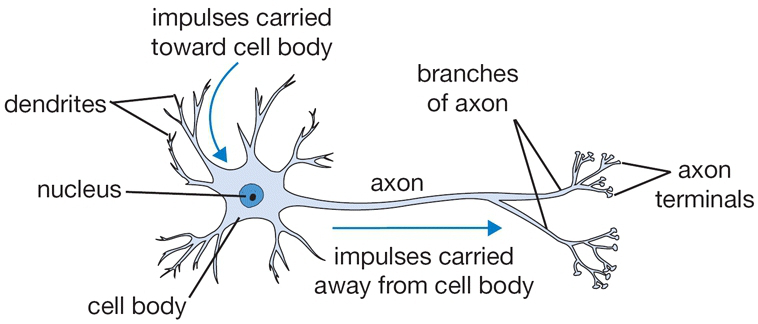
\includegraphics[width=0.6\columnwidth]{images/chap2/neuron.png}
    \footcaption{Cấu tạo một neural thần kinh}
    \label{chap2:animal_neural}
    \end{figure}
\end{center}
\footnotetext{Source: \url{http://cs231n.github.io/neural-networks-1/}}



